% ============================================================================
%  Research paper derived from the thesis
%  "Evaluating Coding Agent Quality: Application to Software Design Principles".
%
%  ACM acmart, sigconf: the format used by the closest related studies of agent
%  pull requests (Cynthia et al., MSR 2026; Sawada et al., EASE 2026; Kashif et
%  al., TOSEM). Compile with pdfLaTeX:
%     latexmk -pdf main.tex
%  For a double-blind submission use:  \documentclass[sigconf,review,anonymous]{acmart}
%
%  Every number below comes from the thesis (checked by
%  vibebench/07_verify/verify_thesis_numbers.py) or, for the Java analysable
%  counts by agent and outcome in Table 1, from
%  vibebench/corpus/java_pr_results.parquet (status == "ok").
%
%  Fields in [square brackets] in the author block are placeholders to fill in.
% ============================================================================
\documentclass[sigconf]{acmart}

% No venue yet: remove the template's placeholder conference, copyright and
% reference-format blocks.
\setcopyright{none}
\settopmatter{printacmref=false}
\renewcommand\footnotetextcopyrightpermission[1]{}
\acmConference{}{}{}
\acmDOI{}
\acmISBN{}

\usepackage{booktabs}
\usepackage{multirow}
\usepackage{array}
\usepackage{tikz}
\usetikzlibrary{arrows.meta,positioning,shapes.geometric,fit,backgrounds,calc,decorations.pathreplacing,shadows}

% Colours used by the figures (same values as the thesis).
\definecolor{issatblue}{RGB}{7,45,90}
\definecolor{issatgold}{RGB}{176,141,60}
\definecolor{accentgray}{RGB}{90,90,90}
\definecolor{lightblue}{RGB}{223,232,242}
\definecolor{srpcolor}{RGB}{31,119,180}
\definecolor{ocpcolor}{RGB}{255,127,14}
\definecolor{lspcolor}{RGB}{44,160,44}
\definecolor{ispcolor}{RGB}{214,39,40}
\definecolor{dipcolor}{RGB}{148,103,189}

\newcolumntype{L}[1]{>{\raggedright\arraybackslash}p{#1}}
\newcommand{\RQ}[1]{\textit{RQ#1}}
\newcommand{\blank}[1]{\rule[-2pt]{#1}{0.4pt}}

% Summary box at the end of each analysis.
\newcommand{\summarybox}[1]{%
  \par\smallskip\noindent
  \fcolorbox{black!40}{black!4}{%
    \begin{minipage}{\dimexpr\columnwidth-2\fboxsep-2\fboxrule\relax}
    \small #1
    \end{minipage}}%
  \par\smallskip}

\begin{document}

\title{Do Coding Agents Introduce SOLID Violations? An Empirical Study of Agent Pull Requests in
Java and Python}

% ---------------------------------------------------------------- authors
\author{Akram Ben Fekih}
\affiliation{%
  \institution{ISSAT Sousse, University of Sousse}
  \city{Sousse}
  \country{Tunisia}}
\email{akram.bf.dev@gmail.com}

\author{Maha Khemaja}
\affiliation{%
  \institution{ISSAT Sousse, University of Sousse}
  \city{Sousse}
  \country{Tunisia}}
\email{maha.khemaja@issatso.u-sousse.tn}

\author{[Third Author]}
\affiliation{%
  \institution{[Institution]}
  \city{[City]}
  \country{[Country]}}
\email{[email]}

\renewcommand{\shortauthors}{Ben Fekih et al.}

\begin{abstract}
Coding agents such as Claude Code, GitHub Copilot and OpenAI Codex now submit pull requests to
open-source projects, but they are mostly evaluated on whether their code passes tests. We examine
whether their contributions follow the five SOLID design principles, using 9,191 analysable pull
requests from the AIDev dataset (4,245 in Java and 4,946 in Python, merged, rejected and open). For
each principle we built a deterministic detector and ran it on the repository before and after each
pull request, so that a pull request is charged only with the violations it adds. An LLM judge
labelled 2,475 sampled entities to estimate the precision and recall of each detector, and the Java
detectors were also compared with CK, PMD and DesigniteJava. Two detectors, new import cycles
(Dependency Inversion) and refused bequest (Liskov Substitution), had high precision. The
other three had precision between 0.110 and 0.425 and are used only as screens. Precision-adjusted
estimates suggest that 0.4--4.1\% of Java and 0.3--3.5\% of Python pull requests introduce a
violation of a given principle, while the touched code already contains many more. The number of
files changed was the strongest predictor of a flag, and the only agent difference found in both
languages was a higher Open/Closed flag rate for Claude Code.
\end{abstract}

\ccsdesc[500]{Software and its engineering~Maintaining software}
\ccsdesc[300]{General and reference~Empirical studies}

\keywords{coding agents, SOLID principles, software design, static analysis, mining software
repositories, LLM-as-a-judge}

\maketitle
\pagestyle{plain}

% ============================================================================
\section{Introduction}
\label{sec:intro}

AI coding tools no longer only suggest the next line of code. Agents such as Claude Code, the GitHub
Copilot coding agent and OpenAI Codex take a task, edit several files, run the tests and open a pull
request. The AIDev dataset~\cite{li2025aidev} contains 7,685,281 pull requests opened by such agents
in 957,209 public GitHub repositories. Many of these pull requests are merged, and after a merge most
of the maintenance on agent-written files is done by people~\cite{sawada2026maintenance}. The design
of agent code matters to the projects that accept it.

Most evaluations of coding agents measure functional correctness. HumanEval~\cite{chen2021codex},
BigCodeBench~\cite{zhuo2024bigcodebench} and SWE-bench~\cite{jimenez2024swebench} check whether
generated code passes a test suite, usually for a single function or issue. Passing tests says little
about coupling, cohesion or class hierarchies, and it is a weak predictor of whether maintainers would
accept a change: METR found that roughly half of the agent patches that pass SWE-bench Verified would
not be merged~\cite{metr2026sweverified}. Some recent studies look at structure. Pehlivan et
al.~\cite{pehlivan2025solid} asked language models to detect SOLID violations in curated examples,
Kashif et al.~\cite{beyond2026designissues} scanned projects generated with Cursor for design issues,
SlopCodeBench~\cite{slopcodebench2026} measured erosion over repeated tasks, and
NITR~\cite{zhu2026nitr} asked agents to fix maintainability problems. These studies use curated
examples, benchmark tasks or newly generated projects, or they count tool warnings without checking
how many are real problems. None of the studies we reviewed (Table~\ref{tab:related}) measures each
SOLID principle on real contributions by several agents with a detector whose precision and recall
are reported.

Measuring design in pull requests raises two problems. A pull request changes code that already
exists, so a violation found in the changed files may be older than the pull request. In addition,
the SOLID principles~\cite{martin2000solid,martin2003agile} describe intent (for example, a class
should have one reason to change), while a static detector sees only structure. How well a detector
matches the principle has to be measured before its numbers can be interpreted.

In this study we sampled 14,006 pull requests by Claude Code, GitHub Copilot and OpenAI Codex from
AIDev, including merged, rejected and open ones. After removing those that changed no analysable
source file or whose source trees could not be recovered, 9,191 remained: 4,245 in Java and 4,946 in
Python. We wrote one
deterministic detector per principle and ran it on the repository before and after each pull
request, charging the pull request only with the difference. To estimate how far the detectors can be
trusted, an LLM judge read 2,475 sampled entities and labelled each one with a reason, following the
approach evaluated by Pehlivan et al.~\cite{pehlivan2025solid}. For Java we also compared the
detectors with three existing analysers. We repeated the whole study in Python, where classes are
optional and no compiler checks overrides, and we treat a result as general only when it appears in
both languages. The study addresses two research questions:

\begin{itemize}
\item \RQ{1} (Adherence and differentiation): Do coding agents differ in how well their pull requests
adhere to the five SOLID principles, and how many of the design problems in the code they touch do
they introduce themselves, in Java and in Python?
\item \RQ{2} (Measurability): Can SOLID adherence be measured at repository scale with deterministic
structural detectors, and how well do these detectors agree with an independent reading judge and
with established analysers?
\end{itemize}

\noindent RQ1 is answered by three analyses: differences between agents once change size,
repository and time are taken into account; a comparison of merged and unmerged code; and a
comparison of the violations a pull request introduced with those already present in the code it
touched. Each analysis is carried out in both languages.

Two of the five detectors, new import cycles for Dependency Inversion and refused bequest for Liskov
Substitution, had high precision (in Java, 0.892 for import cycles and 64 of 64 for refused bequest).
The other three had precision between 0.110 and 0.425.
Precision-adjusted estimates suggest that few pull requests introduced a violation, although the
touched code already contained many. Change size accounted for most of the differences between
agents. The one
difference that held in both languages was a higher Open/Closed rate for Claude Code (odds ratio 2.22
in Java and 2.09 in Python). Merged and unreviewed Java code looked the same, while merged Python code
had fewer flags than unmerged Python code.

The main contributions of this paper are:
\begin{itemize}
\item five deterministic SOLID detectors for Java and Python that compare the repository before and
after a pull request;
\item precision and stratum-weighted recall for each detector, a holdout test of two refinements, a
test of both refinements in a second language, and a comparison with CK, PMD and DesigniteJava;
\item a comparison of three agents over 9,191 analysable pull requests in two languages;
\item evidence that the Liskov violations that can occur depend on the compiler (46 of the 51
confirmed Python violations are faults that \texttt{javac} rejects), and that a categorical detector
rule held on a Java holdout while a fitted numeric threshold did not, with the same pattern in small
Python samples.
\end{itemize}

The pipeline, the labels and the analysis scripts are available at [replication package URL].

% ============================================================================
\section{Background and Related Work}
\label{sec:related}

\subsection{SOLID and its detection}

Martin's design principles~\cite{martin2000solid,martin2003agile} are usually grouped under the
acronym SOLID. The Single Responsibility Principle (SRP) says a class should have one reason to
change. The Open/Closed Principle (OCP) says a module should be open for extension and closed for
modification. The Liskov Substitution Principle (LSP) requires that a subtype can be used wherever
its base type is expected. The Interface Segregation Principle (ISP) says clients should not depend
on members they do not use, and the Dependency Inversion Principle (DIP) says modules should depend on
abstractions.

Violations are usually detected through code smells~\cite{fowler1999refactoring,suryanarayana2014smells}
and metric-based detection strategies~\cite{marinescu2004detection}, which combine thresholds on
metrics such as the CK suite~\cite{chidamber1994metrics}, LCOM4~\cite{hitz1995cohesion} and
conceptual cohesion~\cite{marcus2008c3}. Classes involved in antipatterns tend to change more and to
contain more faults~\cite{khomh2012antipatterns}, but Olbrich et al.~\cite{olbrich2010godclass}
found that God Classes are less change-prone and fault-prone than other classes once size is
controlled. Flags from size-based detectors need to be checked against the code.

\subsection{Design quality of AI-generated code}

Pehlivan et al.~\cite{pehlivan2025solid} prompted four language models to detect SOLID violations in
240 validated examples and found SRP the easiest principle to detect and DIP the hardest. Kashif et
al.~\cite{beyond2026designissues} generated projects with Cursor averaging 16,965 lines. The
projects reached 91\% functional correctness but had 1,305 CodeScene and 3,193 SonarQube design
issues. Zhu et al.~\cite{zhu2026smells} report that code volume predicts structural degradation in
AI-generated repositories, which they call a Volume-Quality Inverse Law. SlopCodeBench~\cite{slopcodebench2026}
followed 15 agents through 36 iterative problems and found structural erosion increasing in 77\% of
trajectories. In NITR~\cite{zhu2026nitr}, agents fixed 4.3\% of dependency-control problems and
15.2\% of responsibility-decomposition problems across 21 C\texttt{++} probes. Konrad et
al.~\cite{konrad2026vibe} describe how agents make architectural decisions implicitly, based on how
the prompt is worded. These studies work with benchmark tasks or newly generated projects, mostly in a
single language, and none of them reports SOLID adherence per principle for several agents.

\subsection{Studies of agent pull requests}

Several studies use AIDev~\cite{li2025aidev}. Mazloomzadeh et al.~\cite{mazloomzadeh2026agentic}
compared agentic and human pull requests over time. Cynthia et al.~\cite{cynthia2026postmerge}
analysed 1,210 merged agent bug-fix pull requests in Python with SonarQube and found that
differences between agents mostly disappeared after normalising for code churn. Ben Sghaier et
al.~\cite{bensghaier2026harness} showed that the agent software affects code quality even when the
underlying model is the same, which suggests that agents built on similar models can still differ.
Table~\ref{tab:related} summarises the studies closest to ours and the part of our question each
one leaves open. Our study measures adherence to each SOLID principle, includes rejected and open
pull requests as well as merged ones, covers Java and Python, and reports how valid each detector
is.

\begin{table*}[t]
\caption{Closely related studies and what they leave open for the question of this paper.}
\label{tab:related}
\footnotesize
\begin{tabular}{@{}L{3.3cm}L{4.4cm}L{4.4cm}L{4.6cm}@{}}
\toprule
\textbf{Study} & \textbf{Code studied} & \textbf{What is measured} & \textbf{Open for our question} \\
\midrule
Pehlivan et al.~\cite{pehlivan2025solid} & 240 curated examples, 4 LLMs & LLM detection of SOLID
violations & detection on examples, not agent contributions \\
Kashif et al.~\cite{beyond2026designissues} & projects generated with Cursor & CodeScene and
SonarQube design issues & one tool, no comparison between agents \\
Zhu et al.~\cite{zhu2026smells} & LLM- and agent-driven projects & code and architecture smells &
smells, not principles \\
SlopCodeBench~\cite{slopcodebench2026} & 15 agents on iterative benchmark problems & verbosity and
erosion across checkpoints & benchmark tasks, not SOLID-specific \\
NITR~\cite{zhu2026nitr} & 21 C\texttt{++} probes & maintainability tasks with a structural oracle &
benchmark tasks in one language \\
Cynthia et al.~\cite{cynthia2026postmerge} & 1,210 merged agent bug-fix pull requests (AIDev,
Python) & SonarQube issues introduced by the pull request & merged bug fixes only, no SOLID
measure \\
\midrule
This study & 9,191 merged, rejected and open agent pull requests (AIDev, Java and Python) & five
SOLID detectors, with measured precision and recall & \\
\bottomrule
\end{tabular}
\end{table*}

% ============================================================================
\section{Study Design}
\label{sec:design}

This is an observational study. The unit of analysis is the pull request, and we measure how each pull
request changed the design of the code it touched. This section describes the corpus, the detectors
and the labelling procedure. The analysis specific to each research question is described with its
results in Section~\ref{sec:results}.

\subsection{Corpus}
\label{sec:corpus}

We used the AIDev-7.6M release~\cite{li2025aidev}. The default tables of this release cover only
repositories with more than 100 stars, so we used the complete tables (\texttt{all\_pull\_request}
and \texttt{all\_repository}). We kept pull requests that change Java or Python source files in
repositories with at least 25 stars and a permissive licence (MIT, Apache-2.0, BSD-2-Clause,
BSD-3-Clause, ISC, 0BSD, Unlicense, CC0-1.0 or MPL-2.0). Three agents have enough pull requests in
both languages: Claude Code, GitHub Copilot and OpenAI Codex. Cursor and Devin were left out because
they have too few Java pull requests (94 and 6), and Google Jules because it appears for the first
time in this release, so its attribution cannot be compared with an earlier one.

A pull request is merged, rejected (closed without merging) or still open. In AIDev as a whole,
80.9\% of agent pull requests are merged, 9.5\% are closed without merging and 9.6\% are open. We
over-sampled rejected and open pull requests so that the outcomes could be compared. For each agent,
we drew twice as many merged pull requests as rejected ones. Rejected and open Java pull requests are
scarce, so all eligible ones were included, which gave 6,956 Java pull requests from 1,010
repositories. In Python we drew 1,400 merged, 700 rejected and 250 open pull requests per agent,
stratified by repository so that no repository contributes more than 0.4\% of any agent and outcome
cell. This gave 7,050 Python pull requests from 3,974 repositories. Rates per outcome can be read as
reported, but a rate pooled over outcomes reflects this sampling design and not the AIDev population.

Most rejected pull requests were closed without any review. Only two groups record a judgement by a
maintainer: pull requests where changes were requested, and pull requests that were reviewed and then
closed. We report these groups separately.

\begin{table}[t]
\caption{Analysable pull requests by agent and outcome.}
\label{tab:corpus}
\footnotesize
\setlength{\tabcolsep}{4pt}
\begin{tabular}{@{}llrrrr@{}}
\toprule
\textbf{Language} & \textbf{Agent} & \textbf{Merged} & \textbf{Rejected} & \textbf{Open} & \textbf{Total} \\
\midrule
\multirow{4}{*}{Java}
 & Claude Code    &    603 &    296 & 210 & 1,109 \\
 & GitHub Copilot &  1,491 &    653 & 222 & 2,366 \\
 & OpenAI Codex   &    479 &    228 &  63 &   770 \\
 & \textit{all}   &  2,573 &  1,177 & 495 & 4,245 \\
\midrule
\multirow{4}{*}{Python}
 & Claude Code    &    940 &    540 & 182 & 1,662 \\
 & GitHub Copilot &    885 &    407 & 178 & 1,470 \\
 & OpenAI Codex   &  1,069 &    549 & 196 & 1,814 \\
 & \textit{all}   &  2,894 &  1,496 & 556 & 4,946 \\
\bottomrule
\end{tabular}

\vspace{3pt}
\raggedright\scriptsize Java: 4,245 of 6,956 sampled pull requests, 790 repositories. Python: 4,946
of 7,050 sampled pull requests, 2,921 repositories.
\end{table}

\subsection{Before and after trees}
\label{sec:trees}

For each pull request we need the source tree before and after the change. We tried four methods in
order: (1)~the merge commit and its first parent, (2)~the commits of the pull request, (3)~the
\texttt{refs/pull/N/head} reference and its merge base, and (4)~the base and head commits reported by
the GitHub API. The first method is only available for merged pull requests. Comparisons between
merged and unmerged code use only pull requests recovered with methods 2 to 4.

Table~\ref{tab:corpus} shows the pull requests that could be analysed. Of the Java sample, 2,540 pull
requests changed no production Java file, 150 exceeded the parsing limit, 18 had lost their history
and 3 had no distinct before tree. Of the Python sample, 1,816 changed no Python file that could be
analysed, 232 changed files that could not be resolved to a module, 40 had no distinct before tree,
14 exceeded the parsing limit and 2 could not be archived. This includes 496 Python pull requests
(7.0\% of the sample) whose branch had been deleted, so their source could no longer be retrieved.

\subsection{Fact extraction}

Java files were parsed with JavaParser and its symbol solver (version 3.25.10), without building the
projects. Source roots were inferred from \texttt{package} declarations, and the median share of
resolved supertypes per pull request is 87.0\%. Python files were parsed with the standard
\texttt{ast} module, and base classes and imports were resolved by module path inside the repository.
Both extractors produce the same record of types, members, supertypes, imports and member accesses,
and the detectors read only this record. Apart from the extractors and the thresholds, the two
languages use the same detector code, labelling procedure and statistical model.

\subsection{Detectors}
\label{sec:detectors}

Table~\ref{tab:detectors} summarises the five detectors. Each detector is a pure function of the
extracted facts, so the same tree always produces the same flags. The rules are our operational
definitions. They capture structures that violations of each principle often leave in the code, and
they do not define the principles themselves. Every rate in this paper is therefore a rate for these
detectors.

\begin{table*}[t]
\caption{The five detectors and their thresholds in each language.}
\label{tab:detectors}
\footnotesize
\begin{tabular}{@{}L{1.4cm}L{1.6cm}L{7.0cm}L{3.0cm}L{3.0cm}@{}}
\toprule
\textbf{Principle} & \textbf{Unit} & \textbf{Rule} & \textbf{Java} & \textbf{Python} \\
\midrule
SRP & class (after tree) & One hit per threshold reached by class length, weighted methods, method
count, largest method complexity, largest parameter count and LCOM; flag at $\geq$2 hits, unless
exactly 2 hits and C3~$\geq$~0.4 &
362 / 45 / 20 / 11 / 5 / 0.86 & 250 / 36 / 10 / 12 / 7 / 0.8 \\
\addlinespace
OCP & dispatch chain & A type or tag/value chain (\texttt{if}/\texttt{else if} ladder or
\texttt{switch} on one subject) reaching the branch threshold, not over an enumeration; the pull
request creates or widens it &
type $\geq$3, tag $\geq$8 & type $\geq$3, value $\geq$5 \\
\addlinespace
LSP & override pair & Override compared with the nearest ancestor method that has a real body &
refused bequest, strengthened precondition, weakened postcondition &
refused bequest, widened return; removed, added required or narrowed parameter \\
\addlinespace
ISP & contract & Interface or abstract contract with $\geq$1 abstract member and $\geq$1
implementer in the repository; forced stub: $\geq$2 stubs forming $\geq$ half of an implementer's
members &
new or widened contract of $\geq$13 members, or a forced stub &
two of: $>$7 abstract members, implementer coverage $<$0.75, a forced stub \\
\addlinespace
DIP & pull request & Two modules become mutually reachable in the internal import graph (Tarjan's
strongly connected components), one of them touched &
new cyclic pair through a touched file & new cyclic pair through a touched module \\
\bottomrule
\end{tabular}

\vspace{3pt}
\raggedright\scriptsize SRP thresholds are class lines / weighted methods per class / methods / method
complexity / parameters / LCOM. Each threshold is close to the 90th percentile of its own corpus and
was set before any label existed.
\end{table*}

\paragraph{SRP} A class gets one hit for each of six size, complexity and cohesion thresholds it
reaches. Cohesion is LCOM4~\cite{hitz1995cohesion}: methods are nodes, two methods are connected when
they use the same field or one calls the other, and constructors are left out. With $c$ connected
components and $n$ methods, $\text{LCOM} = (c-1)/(n-1)$. A class is flagged with two or more hits.
The exception is a class with exactly two hits whose conceptual cohesion C3 is at least 0.4. C3 is the
mean cosine similarity between the TF-IDF vectors of the terms in each pair of methods~\cite{marcus2008c3}.
SRP is scored on the after tree, separately for classes the pull request created and existing
classes it edited.

\paragraph{OCP} A dispatch chain is an \texttt{if}/\texttt{else if} ladder or a \texttt{switch}
that branches on one subject. Chains that test types (\texttt{instanceof}, class literals,
\texttt{getClass()}) are flagged from three branches. Chains that test a tag or value are flagged
from eight branches in Java and five in Python. Chains over an enumeration are ignored, since client
code cannot add values to an enumeration. A pull request is flagged when it adds such a chain or adds
branches to one.

\paragraph{LSP} Each overriding method is compared with the nearest ancestor method that has a real
body, because an abstract method has no behaviour that could be refused. The Java compiler already
rules out several faults: a changed parameter list makes an overload, parameter types cannot be
narrowed, and visibility cannot be reduced. The Java detector therefore checks only refused bequest
(the override only throws a refusal exception), a strengthened precondition and a weakened
postcondition. In Python, where no compiler checks overrides, the detector also checks removed
parameters, added required parameters, narrowed parameter types and widened return types.

\paragraph{ISP} In Java, contracts are interfaces and abstract classes. In Python they are subclasses
of \texttt{abc.ABC} with abstract members and \texttt{Protocol} classes. The width of a contract is
its number of abstract members, and each implementer has a stub ratio. The Python flag requires two
signals, so Java and Python ISP rates measure different things and are not compared directly.

\paragraph{DIP} We build the internal import graph before and after the change and find strongly
connected components with Tarjan's algorithm~\cite{tarjan1972scc}. A pull request is flagged when two
modules become mutually reachable and one of them is a file or module the pull request changed.

All thresholds were set close to the 90th percentile of each language's corpus before any labelling
started. After calibration we deleted the results and ran the analysis again, so every flag was
produced with the final thresholds. Percentile thresholds are common in metric-based detection
strategies~\cite{marinescu2004detection}, but a value in the top decile only marks unusual code,
which is not a violation in itself. We therefore treat the thresholds as screening choices and
assess them through the precision and recall measured for RQ2.

\subsection{Before/after comparison}
\label{sec:delta}

For OCP, LSP, ISP and DIP, the detector runs on both trees and only the difference is charged to the
pull request (Figure~\ref{fig:delta}). For LSP, ISP and DIP, which concern relations between units,
a violation is charged when either end of the relation is in a changed file. A pull request that
widens a base type is charged for subclasses it breaks, even in files it did not change.
We call a violation \emph{present} if it exists in the code the pull request touched, whoever wrote
it, and \emph{introduced} if the before/after comparison attributes it to the pull request.

\begin{figure*}[t]
\centering
% Figure: the before/after delta for Dependency Inversion.
% Left: the import graph before the pull request. Right: after it. The pull
% request touches modules a and c (gold rings) and adds one import, c -> a,
% which closes the cycle a -> b -> c -> a. Bottom: the subtraction the detector
% performs, and what is charged. Module positions are the same in both panels
% so the reader compares like with like; labels sit outside every edge.
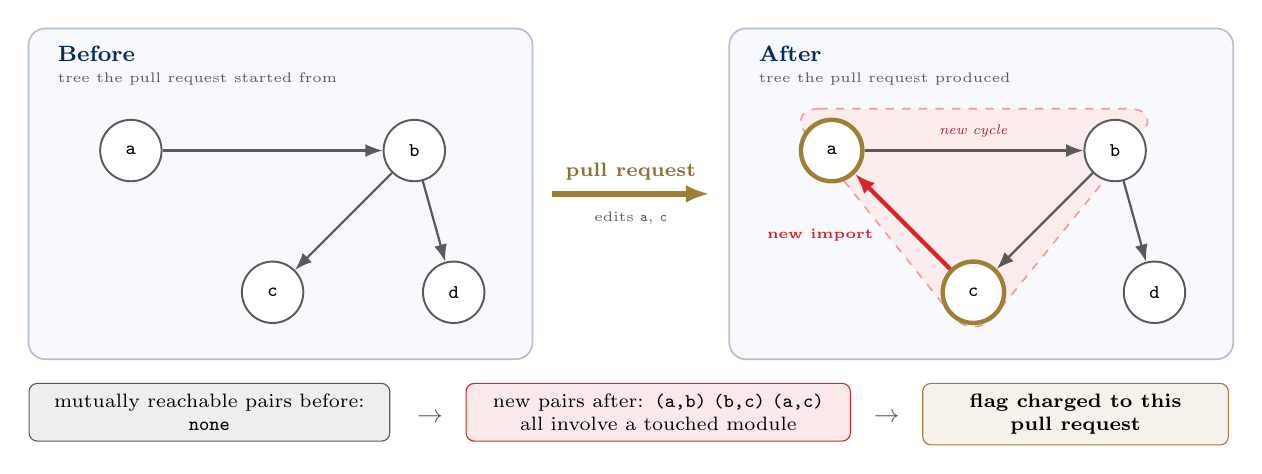
\begin{tikzpicture}[
  font=\scriptsize,
  panel/.style={draw=issatblue!30,fill=lightblue!25,rounded corners=6pt,line width=0.6pt},
  ttl/.style={font=\footnotesize\bfseries,text=issatblue,anchor=west},
  sub/.style={font=\tiny,text=accentgray,anchor=west},
  mod/.style={circle,draw=accentgray,fill=white,line width=0.7pt,minimum size=0.78cm,
              inner sep=0pt,font=\scriptsize\ttfamily},
  touched/.style={mod,draw=issatgold!90!black,line width=1.6pt},
  imp/.style={-{Latex[length=2.2mm]},draw=accentgray,line width=0.8pt},
  newimp/.style={-{Latex[length=2.6mm]},draw=ispcolor,line width=1.5pt},
  cyc/.style={fill=ispcolor!9,draw=ispcolor!45,dashed,line width=0.6pt,rounded corners=12pt},
  chip/.style={draw=#1,fill=#1!10,rounded corners=3pt,inner sep=4pt,align=center,font=\scriptsize},
]
% ---------------------------------------------------------------- panels
\draw[panel] (0,0) rectangle (6.4,-4.2);
\node[ttl] at (0.25,-0.32) {Before};
\node[sub] at (0.25,-0.64) {tree the pull request started from};

\draw[panel] (8.9,0) rectangle (15.3,-4.2);
\node[ttl] at (9.15,-0.32) {After};
\node[sub] at (9.15,-0.64) {tree the pull request produced};

% ------------------------------------------------------------ before graph
\begin{scope}[shift={(0,0)}]
  \node[mod] (a1) at (1.3,-1.55) {a};
  \node[mod] (b1) at (4.9,-1.55) {b};
  \node[mod] (c1) at (3.1,-3.35) {c};
  \node[mod] (d1) at (5.4,-3.35) {d};
  \draw[imp] (a1) -- (b1);
  \draw[imp] (b1) -- (c1);
  \draw[imp] (b1) -- (d1);
\end{scope}

% ------------------------------------------------------------- after graph
\begin{scope}[shift={(8.9,0)}]
  \path[cyc] (0.72,-1.02) -- (5.5,-1.02) -- (3.1,-3.98) -- cycle;
  \node[font=\tiny\itshape,text=ispcolor!80!black,anchor=north] at (3.1,-1.1) {new cycle};
  \node[touched] (a2) at (1.3,-1.55) {a};
  \node[mod] (b2) at (4.9,-1.55) {b};
  \node[touched] (c2) at (3.1,-3.35) {c};
  \node[mod] (d2) at (5.4,-3.35) {d};
  \draw[imp] (a2) -- (b2);
  \draw[imp] (b2) -- (c2);
  \draw[imp] (b2) -- (d2);
  \draw[newimp] (c2) -- (a2);
  \node[font=\tiny\bfseries,text=ispcolor,anchor=east] at (1.95,-2.62) {new import};
\end{scope}

% --------------------------------------------------------- the pull request
\draw[-{Latex[length=3mm]},issatgold!90!black,line width=2pt] (6.65,-2.1) -- (8.65,-2.1);
\node[font=\scriptsize\bfseries,text=issatgold!80!black,anchor=south] at (7.65,-2.05) {pull request};
\node[font=\tiny,text=accentgray,anchor=north,align=center] at (7.65,-2.2) {edits \texttt{a}, \texttt{c}};

% -------------------------------------------------------------- the result
\node[chip=accentgray,anchor=north west,text width=4.3cm] (sub1) at (0,-4.5)
  {mutually reachable pairs before:\\ \texttt{none}};
\node[font=\small,text=accentgray] (minus) at (5.1,-4.95) {$\rightarrow$};
\node[chip=ispcolor,anchor=north west,text width=4.6cm] (res) at (5.55,-4.5)
  {new pairs after: \texttt{(a,b) (b,c) (a,c)}\\all involve a touched module};
\node[font=\small,text=accentgray] at (10.9,-4.95) {$\rightarrow$};
\node[chip=issatgold!90!black,anchor=north west,text width=3.6cm,font=\scriptsize\bfseries] at (11.35,-4.5)
  {flag charged to this\\pull request};
\end{tikzpicture}

\caption{Before/after comparison for Dependency Inversion. The pull request edits modules \texttt{a}
and \texttt{c} and adds the import \texttt{c}$\rightarrow$\texttt{a}, which makes three module pairs
mutually reachable. Only this difference is charged to the pull request.}
\label{fig:delta}
\end{figure*}

\subsection{Labelling}
\label{sec:judge}

For each principle and language we sampled 100 entities the detector flagged and 100 it did not, from
production code (test and generated code excluded), with a fixed seed. An entity touched by several pull requests was counted once. When
a detector flagged few entities, all of them were labelled: the 195 Java DIP flags and the 80 Python
ISP flags. The labels were produced by an LLM of the Claude family used as a
judge~\cite{zheng2023llmjudge}. Java entities were labelled between 5 and 8 September 2026 and
Python entities on 14 September 2026. The judge read the source of each entity (for LSP, the overriding
method next to its base method), did not see the detector's verdict, and returned a yes/no label with
a written reason, following a rubric written before labelling began. In Python, borderline
decisions were recorded as numbered precedents and applied to later entities. The rubric is part of
the replication package. Labels could only be recorded
through a script that rejects a label without a reason or without the source file shown to the
judge, and every batch was checked by an automatic audit before labelling. All precision and recall
values in this paper measure agreement between a detector and this judge.

% ============================================================================
\section{Results}
\label{sec:results}

We report RQ2 first, because the RQ1 analyses use the precision values it produces to adjust flag
counts.

\subsection{RQ2: Measurability}
\label{sec:measure}

\paragraph{Motivation} The SOLID principles are about intent, and the detectors see only structure.
The rates reported for RQ1 are only meaningful if we know how often a flag is a real violation and
how many violations the detectors miss.

\paragraph{Approach} Precision is the share of labelled flags that the judge confirmed. Since each
sample is half flagged and half unflagged while the population is not, recall is weighted by the size
of each stratum. With $N_f$ and $N_u$ the numbers of flagged and unflagged entities in the population
and $n_f$ and $n_u$ the numbers sampled,
\begin{equation}
R = \frac{TP \cdot N_f / n_f}{TP \cdot N_f / n_f + FN \cdot N_u / n_u}.
\label{eq:recall}
\end{equation}
Confidence intervals come from a percentile bootstrap within each stratum. After the first Java
round, we derived two refinements from the false positives: LSP restricted to refused bequest, and
ISP restricted to contracts with at least 30 members. Both were re-scored on a holdout of 200 new
entities drawn with a different seed, excluding every entity labelled before. Both refinements were
fixed before any Python label existed, so the Python labels give a second test. Independently of the
judge, we ran CK~0.7.0~\cite{aniche2015ck}, PMD~7.7.0~\cite{pmd} and
DesigniteJava~1.1.2~\cite{sharma2016designite} with their default settings on the latest tree of 150
randomly chosen Java repositories, and measured agreement with Cohen's
$\kappa$~\cite{cohen1960kappa}, without treating any tool as correct. To check the judge's
consistency, 174 Java entities were labelled twice; the two labels agreed in 89.7\% of cases.

\paragraph{Results} Table~\ref{tab:validation} and Figure~\ref{fig:validation} show how each
detector agreed with the judge on 1,495 Java and 980 Python entities.

\begin{table}[t]
\caption{Detector agreement with the judge. Flagged and unflagged entities were labelled
separately; precision is TP over flagged entities labelled, and recall is weighted by stratum size
(Equation~\ref{eq:recall}).}
\label{tab:validation}
\footnotesize
\setlength{\tabcolsep}{2.6pt}
\begin{tabular}{@{}llrrrrrl@{}}
\toprule
 & & \multicolumn{2}{c}{\textbf{Flagged}} & \multicolumn{2}{c}{\textbf{Unflagged}} & & \\
\cmidrule(lr){3-4}\cmidrule(lr){5-6}
 & \textbf{Principle} & \textbf{n} & \textbf{TP} & \textbf{n} & \textbf{FN} & \textbf{Prec.} & \textbf{Weighted recall} \\
\midrule
\multirow{5}{*}{Java}
 & SRP &  100 &  35 & 100 & 1 & 0.350 & 0.828 (0.579--1.000) \\
 & OCP &  100 &  33 & 100 & 2 & 0.330 & 0.742 (0.512--1.000) \\
 & LSP &  200 &  84 & 200 & 3 & 0.420 & 0.386 (0.210--1.000) \\
 & ISP &  200 &  67 & 200 & 9 & 0.335 & 0.464 (0.331--0.680) \\
 & DIP$^a$ & 195 & 174 & 100 & 0 & 0.892 & 1.000$^b$ \\
\midrule
\multirow{5}{*}{Python}
 & SRP &  100 &  11 & 100 &  0 & 0.110 & 1.000$^b$ \\
 & OCP &  100 &  39 & 100 & 13 & 0.390 & 0.364 (0.257--0.523) \\
 & LSP &  100 &  51 & 100 &  2 & 0.510 & 0.545 (0.315--1.000) \\
 & ISP$^a$ & 80 & 34 & 100 &  0 & 0.425 & 1.000$^b$ \\
 & DIP &  100 & 100 & 100 &  0 & 1.000 & 1.000$^b$ \\
\bottomrule
\end{tabular}

\vspace{3pt}
\raggedright\scriptsize TP: flags the judge confirmed. FN: unflagged entities the judge labelled a
violation. $^a$All flags labelled (195 Java DIP pull requests, 80 Python ISP contracts). $^b$No
unflagged entity was labelled a violation, so no interval is given. Java LSP and ISP include the
holdout round, which doubles their samples.
\end{table}

\begin{figure*}[t]
\centering
% Figure: detector agreement with the reading judge, both languages.
% One row per principle and language. Filled dot = precision; diamond with a
% horizontal whisker = stratum-weighted recall and its 95% Wilson interval; a
% hollow ring = precision of the Java restriction (LSP to refused bequest,
% ISP to >= 30 members), labelled above the ring. Values: Tables tab:validation
% and tab:py-validation. x axis: 0..1 mapped to 11.4 cm starting at x = 2.3;
% the legend sits under the axis title, inside the text width. A dashed diamond
% with no whisker = recall of 1.000 where 0 of 100 unflagged entities were judged
% violations: not a measured interval, only the absence of a found violation.
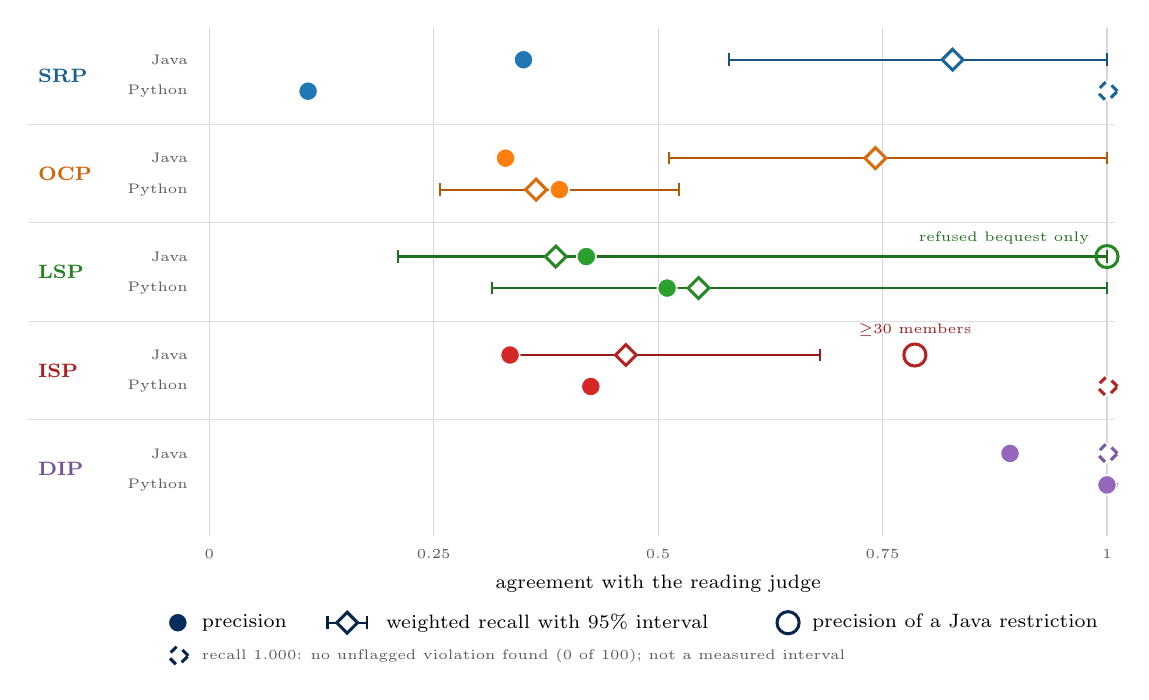
\begin{tikzpicture}[
  font=\scriptsize,
  grid/.style={draw=accentgray!25,line width=0.4pt},
  prec/.style={circle,fill=#1,draw=white,line width=0.6pt,inner sep=0pt,minimum size=7pt},
  rec/.style={diamond,fill=white,draw=#1!85!black,line width=1.1pt,inner sep=0pt,minimum size=8pt},
  ring/.style={circle,draw=#1!85!black,line width=1.1pt,fill=none,inner sep=0pt,minimum size=8pt},
  recz/.style={diamond,fill=white,draw=#1!85!black,dashed,line width=1.1pt,inner sep=0pt,minimum size=8pt},
  whisk/.style={draw=#1!70!black,line width=0.8pt},
  lang/.style={font=\tiny,text=accentgray,anchor=east},
  pname/.style={font=\scriptsize\bfseries,anchor=west},
]
\def\xo{2.3}\def\xs{11.4}
\newcommand{\vrow}[7]{% #1 y, #2 colour, #3 language, #4 precision, #5 recall, #6 lo, #7 hi
  \node[lang] at (\xo-0.15,#1) {#3};
  \draw[whisk=#2] ({\xo+\xs*#6},#1-0.08) -- ({\xo+\xs*#6},#1+0.08);
  \draw[whisk=#2] ({\xo+\xs*#6},#1) -- ({\xo+\xs*#7},#1);
  \draw[whisk=#2] ({\xo+\xs*#7},#1-0.08) -- ({\xo+\xs*#7},#1+0.08);
  \node[rec=#2] at ({\xo+\xs*#5},#1) {};
  \node[prec=#2] at ({\xo+\xs*#4},#1) {};
}
\newcommand{\vrowz}[4]{% #1 y, #2 colour, #3 language, #4 precision; recall 1.000, no unflagged violation found
  \node[lang] at (\xo-0.15,#1) {#3};
  \node[recz=#2] at ({\xo+\xs*1.0},#1) {};
  \node[prec=#2] at ({\xo+\xs*#4},#1) {};
}
% ------------------------------------------------------------------ axis
\foreach \v in {0,0.25,0.5,0.75,1}{
  \draw[grid] ({\xo+\xs*\v},0.4) -- ({\xo+\xs*\v},-6.05);
  \node[font=\tiny,text=accentgray,anchor=north] at ({\xo+\xs*\v},-6.1) {\v};
}
\node[font=\scriptsize,anchor=north] at ({\xo+\xs*0.5},-6.42) {agreement with the reading judge};

\foreach \y/\c/\n in {0/srpcolor/SRP,-1.25/ocpcolor/OCP,-2.5/lspcolor/LSP,-3.75/ispcolor/ISP,-5.0/dipcolor/DIP}{
  \node[pname,text=\c!80!black] at (0,\y-0.2) {\n};
}
\foreach \y in {-0.82,-2.07,-3.32,-4.57}{
  \draw[accentgray!20,line width=0.4pt] (0,\y) -- ({\xo+\xs+0.1},\y);
}
\vrow{0}{srpcolor}{Java}{0.350}{0.828}{0.579}{1.000}
\vrowz{-0.4}{srpcolor}{Python}{0.110}
\vrow{-1.25}{ocpcolor}{Java}{0.330}{0.742}{0.512}{1.000}
\vrow{-1.65}{ocpcolor}{Python}{0.390}{0.364}{0.257}{0.523}
\vrow{-2.5}{lspcolor}{Java}{0.420}{0.386}{0.210}{1.000}
\vrow{-2.9}{lspcolor}{Python}{0.510}{0.545}{0.315}{1.000}
\vrow{-3.75}{ispcolor}{Java}{0.335}{0.464}{0.331}{0.680}
\vrowz{-4.15}{ispcolor}{Python}{0.425}
\vrowz{-5.0}{dipcolor}{Java}{0.892}
\vrowz{-5.4}{dipcolor}{Python}{1.000}

% Java restrictions
\node[ring=lspcolor] (rl) at ({\xo+\xs*1.000},-2.5) {};
\node[font=\tiny,text=lspcolor!70!black,anchor=south east,inner sep=1pt] at ([xshift=-2pt]rl.north west) {refused bequest only};
\node[ring=ispcolor] (ri) at ({\xo+\xs*0.786},-3.75) {};
\node[font=\tiny,text=ispcolor!70!black,anchor=south,inner sep=1pt] at ([yshift=1pt]ri.north) {$\geq$30 members};

% ---------------------------------------------------------------- legend
\begin{scope}[shift={(\xo-0.4,-7.15)}]
  \node[prec=issatblue] at (0,0) {};
  \node[anchor=west] at (0.18,0) {precision};
  \draw[whisk=issatblue] (1.9,0) -- (2.4,0);
  \draw[whisk=issatblue] (1.9,-0.08) -- (1.9,0.08);
  \draw[whisk=issatblue] (2.4,-0.08) -- (2.4,0.08);
  \node[rec=issatblue] at (2.15,0) {};
  \node[anchor=west] at (2.52,0) {weighted recall with 95\% interval};
  \node[ring=issatblue] at (7.75,0) {};
  \node[anchor=west] at (7.93,0) {precision of a Java restriction};
  \node[recz=issatblue] at (0,-0.42) {};
  \node[anchor=west,font=\tiny,text=accentgray] at (0.18,-0.42)
    {recall 1.000: no unflagged violation found (0 of 100); not a measured interval};
\end{scope}
\end{tikzpicture}

\caption{Detector precision and stratum-weighted recall against the judge, in Java and Python. Hollow
rings show the precision of the two Java refinements.}
\label{fig:validation}
\end{figure*}

\paragraph{Dependency Inversion} All 195 Java flags were labelled, so the Java precision of 0.892 (174
of 195) is the value for the whole corpus, not an estimate. In Python, each of the 100 labelled flags
closes a new import cycle through changed code. This shows that the cycles exist, not that every one
of them is harmful.

\paragraph{Liskov Substitution} The three Java signals differ in precision. Refused bequest was correct on 31
of 31 flags in the first sample and 33 of 33 in the holdout, 64 of 64 overall (1.000, 95\% interval
0.943--1.000). Weakened postcondition was correct on 6 of 36 flags and strengthened precondition on 3
of 33. The Python detector, with five signals, reached 0.510. In 46 of its 51 true positives the
violation is a removed parameter, an added required parameter or a narrowed parameter type, all of
which \texttt{javac} would reject. The refused-bequest rule, applied to Python without changes, was
correct on six of seven flags.

\paragraph{Interface Segregation} Java precision depends on contract width: 0.116 for up to 17
members, 0.071 for 18 to 29, 0.786 for 30 to 49 and 0.900 for 50 to 99. A minimum of 30 members gave
0.862 (25 of 29) on the sample it was derived from, but 0.704 (19 of 27) on the holdout, which is
outside the holdout's interval of 0.515--0.841, and 0.200 (1 of 5) in Python. A possible
explanation lies in the form of the two rules. Refused bequest is a yes/no property of a method body,
while the value 30 was chosen where the false positives in one sample stopped, so it may partly fit
the noise in that sample. The Python figures rest on 7 and 5 flags and only point in the same
direction.

\paragraph{Open/Closed} Precision does not depend on the length of the chain. Across five bands of
branch count it stays between 0.270 and 0.400. Most false positives switch over sets that are fixed
by an external specification, such as JDBC type codes, protobuf scalar types, Unicode blocks or
generated parser tables. The compiler treats these sets as open, so the enumeration rule does not
suppress them.

\paragraph{Single Responsibility} Precision is 0.350 in Java and 0.110 in Python. Most of the 89
Python false positives are classes whose size is dictated by a framework, such as model heads in the
\texttt{transformers} library, Home Assistant entities and Lightning callbacks.

\paragraph{Recall} In Java the SRP, OCP and DIP detectors miss few violations (weighted recall 0.742
to 1.000), so their flag rates are upper bounds on what the judge would confirm. The LSP and ISP
detectors have lower recall, 0.386 and 0.464. The three Liskov violations among unflagged Java
entities do not throw where the detector looks: one override throws for every non-null argument,
one has an empty body, and one discards its argument. The weighting matters. For Java LSP the
population contains 574 flagged and 25,594 unflagged override pairs, and without weighting the
recall would be 0.966.

\paragraph{Precision by agent} Table~\ref{tab:agentprec} shows precision for each agent. In Java,
Claude Code's flags were confirmed more often than Copilot's for four of the five principles, the
exception being DIP (0.792 against 0.959). In Python, Claude Code's Open/Closed flags, which carry the
agent difference reported in Section~\ref{sec:agents}, had the highest precision of the three
agents. Because the judge
and Claude Code come from the same model family, we looked for signs of leniency. A lenient judge
would confirm fewer of Claude Code's flags, and we did not see this.

\begin{table}[t]
\caption{Precision by agent: confirmed flags over labelled flags.}
\label{tab:agentprec}
\footnotesize
\setlength{\tabcolsep}{3.4pt}
\begin{tabular}{@{}lcccccc@{}}
\toprule
 & \multicolumn{3}{c}{\textbf{Java}} & \multicolumn{3}{c}{\textbf{Python}} \\
\cmidrule(lr){2-4}\cmidrule(lr){5-7}
\textbf{Principle} & \textbf{Claude} & \textbf{Copilot} & \textbf{Codex} & \textbf{Claude} & \textbf{Copilot} & \textbf{Codex} \\
\midrule
SRP & 18/55  & 10/38 & 7/7   & 6/46  & 2/26  & 3/28 \\
OCP & 23/68  & 7/25  & 3/7   & 20/45 & 7/19  & 12/36 \\
LSP & 53/106 & 22/68 & 9/26  & 29/73 & 11/15 & 11/12 \\
ISP & 35/83  & 26/93 & 6/24  & 23/48 & 6/17  & 5/15 \\
DIP & 57/72  & 94/98 & 23/25 & 53/53 & 16/16 & 31/31 \\
\bottomrule
\end{tabular}
\end{table}

\paragraph{Comparison with existing tools} Table~\ref{tab:tools} compares each Java detector with
the closest rule or smell in the three tools. Over 82,553 production types, our SRP rubric agreed
with PMD's \texttt{GodClass} rule at $\kappa = 0.574$ and with DesigniteJava's \emph{Insufficient
Modularization} and \emph{Multifaceted Abstraction} smells at 0.531, while PMD and DesigniteJava
agreed with each other at 0.384. Of the rubric's 6,326 flags, 4,304 (68.0\%) were also flagged by at
least one of the tools. Our size metrics correlated strongly with CK (Spearman $\rho = 0.977$ for
weighted methods and 0.944 for lines of code), but cohesion did not (0.288 with CK's LCOM1, and CK's
own two variants correlate at only 0.490). The Open/Closed detector found little support. Over 63,326
types in 138 repositories, it flagged 886 types (1.40\%) and DesigniteJava's type-conditional smells
flagged 299 (0.47\%), with 76 types in common ($\kappa = 0.122$). For OCP, the judge is effectively
the only check. The LSP and DIP differences come from how the units are defined. DesigniteJava
reports a broken substitution on the supertype and a cycle on packages, while our detectors report
the subclass and the compilation units. When our DIP flags are grouped by package, their recall
against DesigniteJava is 0.924.

\begin{table}[t]
\caption{Agreement of the Java detectors with existing analysers (Cohen's $\kappa$).}
\label{tab:tools}
\footnotesize
\setlength{\tabcolsep}{3.5pt}
\begin{tabular}{@{}lL{3.5cm}L{2.85cm}@{}}
\toprule
\textbf{Principle} & \textbf{Compared with} & \textbf{$\kappa$} \\
\midrule
SRP & PMD \texttt{GodClass}; DesigniteJava modularization smells & 0.574; 0.531 (the two tools with each other: 0.384) \\
OCP & DesigniteJava \emph{Missing Hierarchy}, \emph{Unexploited Encapsulation} & 0.122 \\
LSP & DesigniteJava \emph{Rebellious Hierarchy} & 0.000 (the tool reports the supertype, we report the subclass) \\
ISP & no counterpart in the three tools & not computable \\
DIP & DesigniteJava cyclic dependency & 0.389 by compilation unit; 0.080 by package \\
\bottomrule
\end{tabular}
\end{table}

\summarybox{\textit{Answer to RQ2.} Partly, and the answer differs by principle. The DIP detector
(new import cycles) and the refused-bequest rule for LSP have high precision in both languages. The SRP, OCP and ISP detectors have
precision between 0.110 and 0.425, so their flags point to code that needs a closer look and should
not be counted as violations. The SRP rubric agrees with published God Class detectors about as well
as they agree with each other, while the OCP detector agrees with none of the tools.}

\subsection{RQ1: Adherence and differentiation}
\label{sec:rq1}

RQ1 has three parts: how the agents differ (Section~\ref{sec:agents}), whether merged code differs
from unmerged code (Section~\ref{sec:outcome}), and how many of the violations in the touched code a
pull request introduced (Section~\ref{sec:locus}).

\subsubsection{Differences between agents}
\label{sec:agents}

\paragraph{Motivation} Teams choosing a coding agent may want to know whether the agents differ in
the structure of the code they contribute, and whether such a difference comes from the agent or
from the kind of change it makes.

\paragraph{Approach} We report flag rates per agent as the average over repositories (macro) and
pooled over all pull requests, because one large repository can dominate a pooled rate. Proportions
have Wilson intervals~\cite{wilson1927interval}. To separate the agent from change size, repository
and time, we fitted for each principle and language the model
\begin{align}
\operatorname{logit}\Pr(\text{flag}) = {} & \beta_0 + \beta_{\text{agent}} \nonumber \\
 & + \beta_1 \log(1 + \text{files}) + \beta_2\,\text{months},
\label{eq:model}
\end{align}
using generalised estimating equations~\cite{liang1986gee} with an exchangeable working correlation
within repositories and cluster-robust standard errors. Copilot, the largest Java group, is the
reference agent. Each agent coefficient is compared with a Bonferroni threshold over the agent
coefficients in its language: six in Java ($0.05/6 = 0.0083$) and ten in Python ($0.05/10 = 0.005$).

\paragraph{Results} Table~\ref{tab:rates} gives the flag rates. Claude Code has the highest pooled
rate for every principle in both languages.

\begin{table}[t]
\caption{Flag rate by agent (\%): average over repositories, with the pooled rate in brackets.}
\label{tab:rates}
\footnotesize
\setlength{\tabcolsep}{3.2pt}
\begin{tabular}{@{}llccc@{}}
\toprule
 & \textbf{Principle} & \textbf{Claude Code} & \textbf{Copilot} & \textbf{Codex} \\
\midrule
\multirow{6}{*}{Java}
 & PRs & 1,109 & 2,366 & 770 \\
 & SRP$^a$ & 8.4 (9.5)   & 3.5 (5.1) & 7.4 (6.8) \\
 & OCP & 10.1 (10.6) & 3.0 (6.4) & 2.2 (2.1) \\
 & LSP$^b$ & 0.3 (0.7) & 0.1 (0.3) & 0.0 (0.0) \\
 & ISP & 6.0 (8.7)   & 4.0 (6.7) & 5.0 (2.9) \\
 & DIP & 5.1 (6.5)   & 2.8 (4.1) & 5.4 (3.2) \\
\midrule
\multirow{6}{*}{Python}
 & PRs & 1,662 & 1,470 & 1,814 \\
 & SRP$^a$ & 11.0 (9.6) & 10.3 (6.6) & 8.1 (8.9) \\
 & OCP & 9.6 (9.7)   & 3.1 (3.5) & 6.6 (5.7) \\
 & LSP & 1.2 (1.6)   & 0.3 (0.5) & 0.8 (0.8) \\
 & ISP & 1.0 (1.3)   & 0.4 (0.4) & 0.1 (0.3) \\
 & DIP & 5.6 (5.8)   & 1.5 (2.0) & 2.3 (2.6) \\
\bottomrule
\end{tabular}

\vspace{3pt}
\raggedright\scriptsize $^a$Over classes created by the agent; other rows over pull requests.
$^b$Refused bequest only, the rule used for Java (16 pull requests in total).
\end{table}

The agents make changes of very different sizes. On average a pull request touches 46.4 files for
Claude Code, 18.5 for Copilot and 10.9 for Codex in Java, and 16.5, 7.7 and 9.6 files in Python. Flag
rates increase with size for every agent, which is expected for detectors that compare two trees: a
larger change gives them more opportunities to fire. When Java pull requests are grouped by size, the
ordering of the agents only holds for the largest changes. Among pull requests that touch 11 or more
files, 31.3\% of Claude Code's are flagged for OCP, compared with 8.9\% of Codex's. Among pull
requests that touch three files or fewer, Copilot has the highest OCP and ISP rates and Codex the
highest DIP rate.

Table~\ref{tab:model} shows the fitted model. Change size is the strongest term for every principle
in both languages. Each doubling of the number of files touched multiplies the odds of a flag by 1.88
to 1.95 in Java and by 2.01 to 2.18 in Python ($p < 10^{-4}$).

\begin{table*}[t]
\caption{Adjusted odds ratios with 95\% confidence intervals (reference agent: GitHub Copilot).}
\label{tab:model}
\footnotesize
\begin{tabular}{@{}llccccc@{}}
\toprule
 & \textbf{Term} & \textbf{SRP} & \textbf{OCP} & \textbf{LSP} & \textbf{ISP} & \textbf{DIP} \\
\midrule
\multirow{5}{*}{Java}
 & Claude Code      & n/a$^a$ & 2.22 (1.21--4.07) & n/a$^b$ & 1.11 (0.63--1.95) & 1.29 (0.50--3.36) \\
 & OpenAI Codex     & n/a$^a$ & 0.57 (0.24--1.37) & n/a$^b$ & 0.72 (0.40--1.32) & 1.68 (0.79--3.56) \\
 & Size, per doubling & n/a$^a$ & 1.89 (1.75--2.04) & n/a$^b$ & 1.88 (1.73--2.04) & 1.95 (1.77--2.16) \\
 & Time, per month  & n/a$^a$ & 1.00 (0.91--1.10) & n/a$^b$ & 1.02 (0.95--1.10) & 1.03 (0.93--1.15) \\
 & Flagged / total  & n/a$^a$ & 286 / 4,245 & 16 / 4,245 & 276 / 4,245 & 195 / 4,245 \\
\midrule
\multirow{5}{*}{Python}
 & Claude Code      & 1.09 (0.93--1.29) & 2.09 (1.44--3.04)$^\dagger$ & 1.81 (0.74--4.42) & 1.71 (0.67--4.36) & 1.88 (1.17--3.03) \\
 & OpenAI Codex     & 1.06 (0.90--1.25) & 1.46 (0.98--2.16) & 1.38 (0.54--3.52) & 0.53 (0.16--1.80) & 1.12 (0.67--1.86) \\
 & Size, per doubling & 2.06 (1.94--2.18) & 2.01 (1.88--2.15) & 2.18 (1.89--2.51) & 2.17 (1.82--2.58) & 2.04 (1.89--2.21) \\
 & Time, per month  & 1.05 & 0.99 & 0.96 & 0.94 & 1.06 \\
 & Flagged / total  & 2,532 / 4,946 & 315 / 4,946 & 47 / 4,946 & 32 / 4,946 & 173 / 4,946 \\
\bottomrule
\end{tabular}

\vspace{3pt}
\raggedright\scriptsize $^a$Java SRP is scored per class, so there is no pull-request flag to model;
created and edited classes are compared in Section~\ref{sec:locus}. $^b$Not fitted, because only 16
pull requests are flagged. $^\dagger$The only agent coefficient that passes the Bonferroni threshold
of its language (Java $0.05/6 = 0.0083$, Python $0.05/10 = 0.005$); Java OCP for Claude Code has
$p = 0.010$ and Python DIP for Claude Code $p = 0.0096$. Java model: 790 repositories; Python model:
2,921.
\end{table*}

Only one agent effect appears in both languages. Claude Code's odds of an OCP flag are 2.22 times
Copilot's in Java (1.21--4.07, $p = 0.010$) and 2.09 times in Python (1.44--3.04, $p = 0.0001$).
The Java estimate on its own does not pass the Bonferroni threshold of 0.0083, but the Python estimate
passes 0.005, and the two estimates are close. We therefore consider this difference supported. In
Python, Claude Code also has higher odds of introducing an import cycle (1.88, 1.17--3.03,
$p = 0.0096$). This estimate does not pass the Bonferroni threshold, and the Java estimate (1.29) has
an interval that includes 1, so we do not treat it as confirmed. All other agent coefficients have
intervals that include 1.

Time had no detectable effect on the before/after principles in either language. The Python SRP flag
at pull-request level increases by 5\% per month ($p < 10^{-4}$). Since this flag has a precision of
0.110, the trend tells us that large classes are touched or created more often over time, not that
responsibility violations are increasing.

\subsubsection{Merged and unmerged code}
\label{sec:outcome}

\paragraph{Motivation} Most studies of agent code use only merged pull requests. If maintainers tended
to reject structurally worse code, results from merged code would partly reflect the reviewers'
choices.

\paragraph{Approach} We compared only pull requests recovered with methods 2 to 4, so that merged and
unmerged pull requests obtain their before tree in the same way, and we split unmerged pull requests
by how they were closed. In Python we also added an indicator for unmerged pull requests to the
model in Equation~\eqref{eq:model}.

\paragraph{Results} Table~\ref{tab:outcome} gives the flag rates for each group.

\begin{table}[t]
\caption{Flag rate (\%) by outcome, for pull requests recovered with methods 2 to 4.}
\label{tab:outcome}
\footnotesize
\setlength{\tabcolsep}{3.3pt}
\begin{tabular}{@{}llrcccc@{}}
\toprule
 & \textbf{Outcome} & \textbf{n} & \textbf{OCP} & \textbf{LSP} & \textbf{ISP} & \textbf{DIP} \\
\midrule
\multirow{5}{*}{Java}
 & merged               & 1,521 & 8.3  & 0.5 & 7.5  & 4.6 \\
 & changes requested    &    36 & 5.6  & 0.0 & 16.7 & 13.9 \\
 & reviewed, closed     &   135 & 12.6 & 0.7 & 12.6 & 12.6 \\
 & closed unreviewed    & 1,006 & 7.5  & 0.5 & 5.5  & 5.6 \\
 & open                 &   490 & 8.8  & 0.2 & 9.2  & 5.9 \\
\midrule
\multirow{5}{*}{Python}
 & merged               & 1,734 & 4.9  & 0.5 & 0.4 & 3.1 \\
 & changes requested    &    33 & 9.1  & 0.0 & 0.0 & 9.1 \\
 & reviewed, closed     &   163 & 7.4  & 1.2 & 1.8 & 8.6 \\
 & closed unreviewed    & 1,300 & 9.1  & 1.7 & 0.9 & 4.5 \\
 & open                 &   553 & 10.8 & 2.2 & 1.1 & 5.2 \\
\bottomrule
\end{tabular}

\vspace{3pt}
\raggedright\scriptsize SRP is scored per class and is not split by outcome. Python flagged counts
for merged pull requests: OCP 85, LSP 8, ISP 7, DIP 54.
\end{table}

In Java, merged pull requests and the 1,006 pull requests closed without review have rates within two
percentage points of each other for every principle. The two reviewed groups have higher ISP and DIP
rates. For pull requests that were reviewed and then closed, the Wilson interval for DIP
(8.0--19.2\%) does not overlap the interval for merged code (3.7--5.8\%). These groups are small,
however, and 6 of the 17 flagged pull requests in the reviewed-then-closed group come from one
repository.

In Python, merged pull requests have lower rates than the unreviewed, reviewed-then-closed and open
groups for all four principles. For OCP, for example, the rate is 4.9\% for merged pull requests and
9.1\% for the 1,300 closed without review. Unmerged pull requests are larger (median four files
compared with three). After adjusting for size and agent, with repository clustering, unmerged pull
requests still have higher odds of an OCP flag (1.57, 1.15--2.15, $p = 0.004$) and of an LSP flag
(2.43, 1.08--5.46, $p = 0.03$). For ISP (1.71, 0.75--3.91) and DIP (1.36, 0.92--2.03) the difference
is not significant.

\subsubsection{Present and introduced violations}
\label{sec:locus}

\paragraph{Motivation} A violation in the code an agent touched was not necessarily written by the
agent. Comparing the violations a pull request introduced with those already present shows whether
agents create design problems or mostly work in code that already has them.

\paragraph{Approach} The present count is the number of distinct flagged production entities in the
touched code. The introduced count is the number of pull requests whose before/after comparison adds
a violation. Multiplying both counts by the detector's precision gives precision-adjusted estimates.
These assume that the precision measured on the sample holds for the whole corpus, and they carry
the uncertainty of that measurement. For SRP we compare classes created by the agents with existing
classes they edited.

\paragraph{Results} Table~\ref{tab:present} and Figure~\ref{fig:present} compare the two counts.

\begin{table}[t]
\caption{Violations present in the touched code and pull requests that introduced one.}
\label{tab:present}
\footnotesize
\setlength{\tabcolsep}{2.4pt}
\begin{tabular}{@{}lrrrr@{}}
\toprule
 & \multicolumn{2}{c}{\textbf{Java}} & \multicolumn{2}{c}{\textbf{Python}} \\
\cmidrule(lr){2-3}\cmidrule(lr){4-5}
\textbf{Principle} & \textbf{Present (adj.)} & \textbf{Introd.} & \textbf{Present (adj.)} & \textbf{Introd.} \\
\midrule
SRP$^a$ & 7,501 ($\approx$2,600) & n/a & 8,208 ($\approx$900) & 449 (1.0\%) \\
OCP & 2,343 ($\approx$770) & 286 (2.2\%) & 2,580 ($\approx$1,000) & 315 (2.5\%) \\
LSP$^b$ & 183 (183) & 16 (0.4\%) & 176 & 5 \\
ISP & 816 ($\approx$270) & 276 (2.2\%) & 80 (34) & 32 (0.3\%) \\
DIP$^c$ & 195 (174) & 195 (4.1\%) & 173 ($\approx$173) & 173 (3.5\%) \\
\bottomrule
\end{tabular}

\vspace{3pt}
\raggedright\scriptsize Present: distinct flagged production entities in the touched code, with the
precision-adjusted estimate in brackets. Introduced: flagged pull requests, with the
precision-adjusted share of all analysable pull requests in brackets. $^a$Classes; Java has no
introduced count because its SRP flag is per class. $^b$Refused-bequest relationships in both
languages; with all five Python signals, 2,069 override pairs ($\approx$1,050 adjusted) and 47 pull
requests (0.5\%).
$^c$The detector records only new cycles, so both counts are pull requests.
\end{table}

\begin{figure*}[t]
\centering
% Figure: violations present in touched production code (grey dot) against pull
% requests that introduced one (coloured dot), log scale, both languages.
% Present = distinct flagged production entities (samplers' population);
% introduced = flagged pull requests. The LSP row uses refused bequest in both
% languages so the two are comparable. DIP records only new cycles, so the two
% counts coincide and a single dot is drawn. Java SRP has no introduced count.
% Rows follow the thesis order S, O, L, I, D.
% Values: Java SRP 7,501 / -, OCP 2,343 / 286, LSP 183 / 16, ISP 816 / 276,
% DIP 195; Python SRP 8,208 / 449, OCP 2,580 / 315, LSP 176 / 5, ISP 80 / 32,
% DIP 173. Checked by verify_thesis_numbers.py where the thesis states them.
% x = 2.3 + 2.5 * log10(count): 1 .. 10,000 over 10 cm.
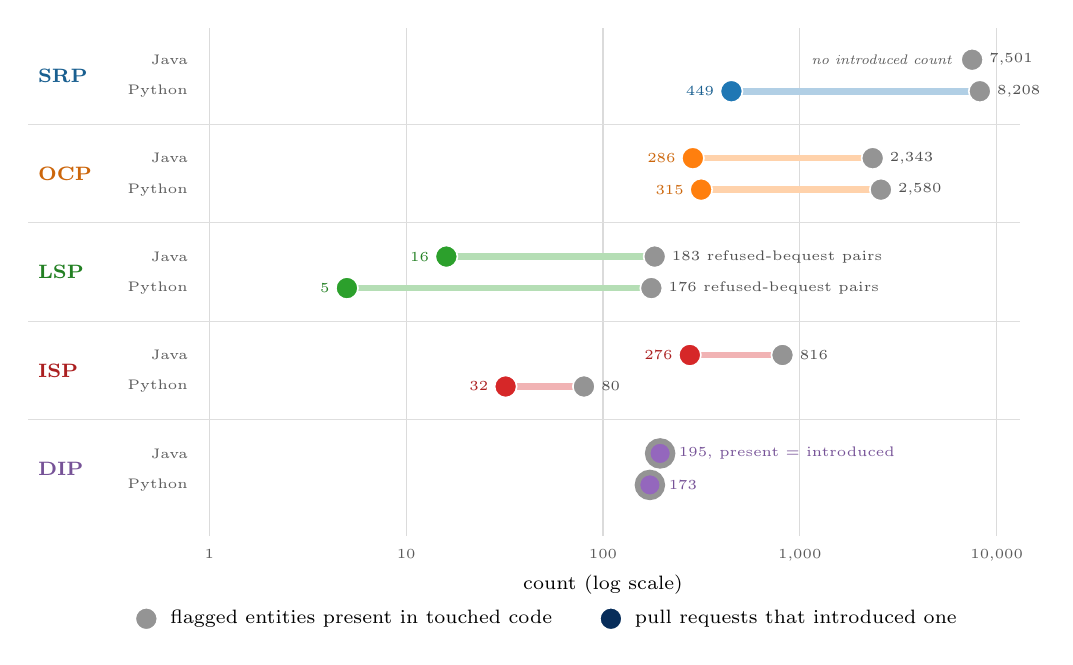
\begin{tikzpicture}[
  font=\scriptsize,
  grid/.style={draw=accentgray!22,line width=0.4pt},
  bell/.style={draw=#1!35,line width=2.4pt,line cap=round},
  pres/.style={circle,fill=accentgray!65,draw=white,line width=0.6pt,inner sep=0pt,minimum size=8pt},
  intro/.style={circle,fill=#1,draw=white,line width=0.6pt,inner sep=0pt,minimum size=8pt},
  both/.style={circle,fill=#1,draw=accentgray!65,line width=2pt,inner sep=0pt,minimum size=9pt},
  val/.style={font=\tiny,inner sep=1.5pt},
  lang/.style={font=\tiny,text=accentgray,anchor=east},
  pname/.style={font=\scriptsize\bfseries,anchor=west},
]
\def\xo{2.3}
\newcommand{\X}[1]{{\xo+2.5*log10(#1)}}
\newcommand{\pair}[6]{% #1 y, #2 colour, #3 language, #4 present, #5 introduced, #6 present label
  \node[lang] at (\xo-0.15,#1) {#3};
  \draw[bell=#2] (\X{#5},#1) -- (\X{#4},#1);
  \node[pres] at (\X{#4},#1) {};
  \node[intro=#2] at (\X{#5},#1) {};
  \node[val,anchor=west,text=accentgray!90!black] at ({\xo+2.5*log10(#4)+0.16},#1) {#6};
  \node[val,anchor=east,text=#2!80!black] at ({\xo+2.5*log10(#5)-0.16},#1) {#5};
}
% axis
\foreach \v/\t in {1/1,10/10,100/100,1000/1{,}000,10000/10{,}000}{
  \draw[grid] (\X{\v},0.4) -- (\X{\v},-6.05);
  \node[font=\tiny,text=accentgray,anchor=north] at (\X{\v},-6.1) {\t};
}
\node[font=\scriptsize,anchor=north] at ({\xo+5},-6.42) {count (log scale)};

\foreach \y/\c/\n in {0/srpcolor/SRP,-1.25/ocpcolor/OCP,-2.5/lspcolor/LSP,-3.75/ispcolor/ISP,-5.0/dipcolor/DIP}{
  \node[pname,text=\c!80!black] at (0,\y-0.2) {\n};
}
\foreach \y in {-0.82,-2.07,-3.32,-4.57}{
  \draw[accentgray!20,line width=0.4pt] (0,\y) -- ({\xo+10.3},\y);
}

% SRP: Java has no introduced count
\node[lang] at (\xo-0.15,0) {Java};
\node[pres] at (\X{7501},0) {};
\node[val,anchor=west,text=accentgray!90!black] at ({\xo+2.5*log10(7501)+0.16},0) {7,501};
\node[val,anchor=east,text=accentgray,font=\tiny\itshape] at ({\xo+2.5*log10(7501)-0.2},0) {no introduced count};
\pair{-0.4}{srpcolor}{Python}{8208}{449}{8,208}

\pair{-1.25}{ocpcolor}{Java}{2343}{286}{2,343}
\pair{-1.65}{ocpcolor}{Python}{2580}{315}{2,580}
\pair{-2.5}{lspcolor}{Java}{183}{16}{183 refused-bequest pairs}
\pair{-2.9}{lspcolor}{Python}{176}{5}{176 refused-bequest pairs}
\pair{-3.75}{ispcolor}{Java}{816}{276}{816}
\pair{-4.15}{ispcolor}{Python}{80}{32}{80}

% DIP: the detector records only new cycles, so present equals introduced
\node[lang] at (\xo-0.15,-5.0) {Java};
\node[both=dipcolor] at (\X{195},-5.0) {};
\node[val,anchor=west,text=dipcolor!80!black] at ({\xo+2.5*log10(195)+0.18},-5.0) {195, present = introduced};
\node[lang] at (\xo-0.15,-5.4) {Python};
\node[both=dipcolor] at (\X{173},-5.4) {};
\node[val,anchor=west,text=dipcolor!80!black] at ({\xo+2.5*log10(173)+0.18},-5.4) {173};

% legend
\begin{scope}[shift={(\xo-0.8,-7.1)}]
  \node[pres] at (0,0) {};
  \node[anchor=west] at (0.18,0) {flagged entities present in touched code};
  \node[intro=issatblue] at (5.9,0) {};
  \node[anchor=west] at (6.08,0) {pull requests that introduced one};
\end{scope}
\end{tikzpicture}

\caption{Flagged violations present in the production code the agents touched (grey) and pull
requests that introduced one (colour), on a log scale. LSP uses refused bequest in both languages.}
\label{fig:present}
\end{figure*}

According to the precision-adjusted estimates, between 0.4\% and 4.1\% of Java pull requests and
between 0.3\% and 3.5\% of Python pull requests introduced a violation of a given principle. The touched code already
contained hundreds to thousands of flagged entities. The difference is largest for the principles
that involve two units. The touched Java code contains 183 refused-bequest relationships, and 16 pull
requests introduced one. In Python the numbers are 176 and five. A refused bequest needs a base
method and an override that contradicts it, an ISP violation needs a contract and its implementers,
and a cycle needs several modules. A single pull request rarely writes both sides of such a relation.
An SRP or OCP violation, by contrast, sits inside one class or one conditional, which a single pull
request can write completely.

The counts for refused bequest are small (16 Java and five Python pull requests), so the
introduction rate for LSP is imprecise and we report it only as an order of magnitude. The LSP
detector also has the lowest recall of the five and undercounts in the 718 Java pull requests with
less than 50\% of supertypes resolved. Both problems mean that more violations are present than we
counted, so the real gap is probably larger.

Classes created by the agents are flagged less often than existing classes they edited. Pooled, the
rates are 7.7\% and 13.5\% in Java (13,712 created and 48,433 edited classes) and 8.9\% and 12.1\% in
Python. Averaged over repositories they are 5.6\% and 20.9\% in Java and 9.7\% and 23.6\% in Python.
New classes also tend to be smaller and younger than existing ones, so this comparison describes the
corpus and should not be read as a comparison between agents and human developers.

\summarybox{\textit{Answer to RQ1.} The agents do introduce SOLID violations, but rarely. The
precision-adjusted share of pull requests that introduce one is 0.4--4.1\% in Java and 0.3--3.5\% in
Python, depending on the principle, while the code they touch already contains many more. Violations
between two units mostly build up over many changes. The agents differ less than raw rates suggest:
change size accounts for most of the differences, and only Claude Code's higher OCP rate holds in
both languages. These are adjusted associations, since the agents worked on different tasks. Merged
code does not differ from unreviewed code in Java but has fewer flags in Python; with only 171 and
196 reviewed rejections, the data cannot show what reviewers base their decisions on.}

% ============================================================================
\section{Discussion}
\label{sec:discussion}

\subsection{Implications for practitioners}

The differences between the three agents are small and mostly related to how much code each agent
changes in one pull request. A SOLID profile can complement functional benchmarks when choosing an
agent, but it does not replace them.

For teams that run automated checks on pull requests, refused bequest is a candidate check. It is
simple to compute and was confirmed on 64 of 64 Java flags and six of seven Python flags. It is also
rare: only 16 of 4,245 Java pull requests introduced one, and we did not measure the recall of this
rule on its own, so it would catch few problems. In Python, a check that an override still accepts
the calls its base method accepts may be more useful, since such faults made up 46 of the 51
confirmed Python Liskov violations. We would not reuse an interface width threshold from another
corpus. Ours lost 16 points on the holdout and was correct on one of five
flags in Python. Size-based SRP flags and branch-count OCP flags are useful as prompts for a
reviewer, but should not block a merge, since most of them were not confirmed by the judge. Problems
between units, which build up over many changes, are hard to see when reviewing one pull request at a
time. Checks that look at the history of a component would be better suited to them.

\subsection{Implications for researchers}

\paragraph{Validating detectors} Detector precision in this study ranged from 0.110 to 1.000. Taking
flags at face value would overstate Python SRP violations about ninefold (11.6\% of touched classes
are flagged, 1.3\% precision-adjusted). For Java LSP, unweighted recall would be 2.5 times the weighted
value (0.966 compared with 0.386). Studies that rely on static detectors should report their
precision and weight recall by the sampled population.

\paragraph{Effect of the language} Three kinds of Liskov fault that made up most of the confirmed
Python violations cannot occur in Java code that compiles. A detector designed for one language may
cover only part of the principle in another, and comparing raw rates across languages mixes differences between agents with
differences between type systems.

\paragraph{Refining detectors} Both refinements were derived from the same Java labels. The rule
based on a code pattern held on the Java holdout and the numeric threshold did not. This is one pair
of rules, so it is weak evidence, but it suggests testing any threshold tuned on labelled false
positives on a fresh sample before using it.

\paragraph{Combining detectors and language models} Pehlivan et al.~\cite{pehlivan2025solid} found
that language models detect SRP violations most easily and DIP violations least easily. Our
structural detectors show the opposite order: DIP has the highest precision (0.892 and 1.000) and SRP
the lowest (0.350 and 0.110). A model reading a short example can judge whether a class does several
things, but it cannot see an import cycle across files it was not shown. A static analyser computes
the whole import graph but cannot judge intent. Using both kinds of detector together might cover
more of the five principles than either one alone; we did not test this. The two studies also differ
in data and setting, so the comparison is indirect.

\subsection{Comparison with earlier studies}

The strong effect of change size is consistent with the Volume-Quality Inverse Law reported by Zhu et
al.~\cite{zhu2026smells}, here observed on real pull requests, in two languages and for all modelled
principles. It also agrees with Cynthia et al.~\cite{cynthia2026postmerge}, who found that
differences between agents in SonarQube issues mostly disappear after normalising for churn, although
we found one difference that remains. The similarity between merged and unreviewed Java code is in
line with METR's observation that passing tests and acceptance by maintainers measure different
things~\cite{metr2026sweverified}. NITR~\cite{zhu2026nitr} found that agents rarely succeed in
repairing dependency structure, and we found that they rarely damage it. The two results are
consistent with agents changing dependency structure little in either direction, although neither
study tests this directly. SlopCodeBench~\cite{slopcodebench2026}
measured erosion over long sequences of edits by the same agent. Our unit is a single pull request,
so our time coefficient does not test that result.

% ============================================================================
\section{Threats to Validity}
\label{sec:threats}

\paragraph{Construct validity} We measure conformity to five principles, not design quality, and we
do not observe outcomes such as defects or maintenance cost. The link between smells and such
outcomes is not uniform~\cite{olbrich2010godclass}. Each detector is a proxy for its principle. The
comparison with existing tools covers only Java and has no counterpart for ISP. The Python ISP flag is defined differently from the Java one, so the raw ISP rates (6.5\% of Java and
0.6\% of Python pull requests) cannot be compared. For Python DIP, the labels confirm that the
flagged cycles exist, not that they are harmful. The detector thresholds are percentile-based
screening choices, and their only support is the precision and recall measured for RQ2.

\paragraph{Internal validity} The agents chose their own tasks in repositories we do not control, so
the model coefficients are adjusted associations and not causal effects. Differences in the tasks
given to each agent remain in its coefficient. Adjusting for change size also removes any part of an
agent's effect that works through the size of its changes. Change size is measured as the number of
files touched. We did not test other measures, such as lines or classes changed, so the size effect
and the adjusted agent differences may depend on this choice. Time is modelled as a linear trend,
which would not detect a sudden change such as a new model release. Symbol resolution is incomplete (median
87.0\% in Java, and only bases inside the repository in Python), which removes candidates and makes
the LSP and ISP rates in RQ1 lower bounds. Because a relation-level violation is charged when
either end is touched, the present counts in Section~\ref{sec:locus} are an upper bound on what the agents could be
responsible for. The outcome comparison in Section~\ref{sec:outcome} uses only methods 2 to 4, since method 1 exists only
for merged pull requests, and it is also affected by the uneven loss of deleted branches described
below.

\paragraph{External validity} Both corpora come from one dataset and from repositories with at least
25 stars and a permissive licence. Repositories above the parsing limit were excluded (150 Java pull
requests). Java and Python both use nominal class hierarchies, so languages with structural typing
are not covered. The Python corpus lost 496 pull requests (7.0\%) because their branches were deleted.
The loss was uneven: 11.0\% of rejected and 5.1\% of merged pull requests, and 14.3\% of Copilot's
pull requests compared with 3.6\% and 3.1\% for the other two agents. We did not replace them, because
replacements could only come from pull requests whose branches still exist. The agents were updated
during the period covered by the data, and the pull requests of each agent come from different
months.

\paragraph{Conclusion validity} Several agent coefficients are tested, so we apply a Bonferroni
correction per language. Counts for the relation-level principles are small (16 Java pull requests
introduce a refused bequest, and 32 Python pull requests are flagged for ISP), which gives wide
intervals. Weighted recall depends on the few violations found in large unflagged strata. Only 171
Java and 196 Python unmerged pull requests were reviewed, which limits what the outcome comparison can say about review.

% ============================================================================
\section{Conclusion}
\label{sec:conclusion}

Within the limits of our detectors, the three coding agents rarely introduced SOLID violations in
the 9,191 pull requests we analysed. The precision-adjusted share of pull requests that introduced a
violation was between 0.3\% and 4.1\% per principle and language, and the code they touched already
contained many more flagged problems. Differences between the agents were mostly accounted for by
the number of files they changed, and only Claude Code's higher OCP rate appeared in both languages.

The main qualification is the strength of the detectors. The evidence is best for import cycles and
refused bequest, which had high precision against the judge. For SRP, OCP and ISP the flags are
screens, and the estimates depend on their measured precision. For automated review,
refused bequest is precise but rare, while size-based and branch-count flags are better treated as
hints for reviewers.

Future work could add a change-history signal for OCP, recognise sets fixed by external
specifications, make the Python SRP screen aware of frameworks, and follow repositories over time to study violations that build up across many pull
requests.

\section*{Data Availability}

The corpus is derived from the public AIDev dataset~\cite{li2025aidev}. The pipeline, configuration,
result tables, the 2,475 labels with their reasons and the scripts that compute every reported number
are kept under version control; the replication package is linked in Section~\ref{sec:intro}.

\section*{Ethics}

The study involves no human participants and no personal data. All repositories were public and had
a permissive licence when they were collected, and they are not redistributed. A language model was
used only to read public source code and label a validation sample. It does not compute any reported
number.

\bibliographystyle{ACM-Reference-Format}
\bibliography{references}

\end{document}
